\documentclass[10pt,letterpaper]{article}
\usepackage[margin=0.75in]{geometry}
\usepackage{amsmath}
\usepackage{amsfonts}
\usepackage{amssymb}
\usepackage{graphicx}
\usepackage{cancel}
\usepackage{listings}
\usepackage{color}
\usepackage{textcomp}
\definecolor{listinggray}{gray}{0.9}
\definecolor{lbcolor}{rgb}{0.9,0.9,0.9}
\lstset{
	backgroundcolor=\color{lbcolor},
	tabsize=4,
	rulecolor=,
	language=Python,
        basicstyle=\scriptsize,
        upquote=true,
        aboveskip={1.5\baselineskip},
        columns=fixed,
        showstringspaces=false,
        extendedchars=true,
        breaklines=true,
        prebreak = \raisebox{0ex}[0ex][0ex]{\ensuremath{\hookleftarrow}},
        frame=single,
        showtabs=false,
        showspaces=false,
        showstringspaces=false,
        identifierstyle=\ttfamily,
        keywordstyle=\color[rgb]{0,0,1},
        commentstyle=\color[rgb]{0.133,0.545,0.133},
        stringstyle=\color[rgb]{0.627,0.126,0.941},
}

\def\mbf{\mathbf}
\def\mbb{\mathbb}

\providecommand{\abs}[1]{\left\lvert#1\right\rvert}
\providecommand{\norm}[1]{\left\lVert#1\right\rVert}
\def\d{\mathrm{d}}
\def\e{\mathrm{e}}

\title{Numerical Treatment of Differential Equations: Homework 10}
\author{Truman Ellis}

\begin{document}
\maketitle

We wish to demonstrate that 
\[
\inf_{p\in Q_{k,k}}\norm{u-p}_{m,2,E}\le Ch^{k+1-m}\abs{u}_{k+1,2,E}
\]
for $k=1$ and both $m=0,1$. Thus we need to show that
\[
\inf_{p\in Q_{1,1}}\norm{u-p}_{0,2,E}\le Ch^2\left(\norm{u_{xx}}_{0,2,E}^2
+\norm{u_{xy}}_{0,2,E}^2+\norm{u_{yy}}_{0,2,E}^2\right)^{\frac{1}{2}}\,,
\]
and
\[
\inf_{p\in Q_{1,1}}\left(
\norm{u-p}_{0,2,E}^2
+\norm{u_x-p_x}_{0,2,E}^2
+\norm{u_y-p_y}_{0,2,E}^2\right)^{\frac{1}{2}}
\le Ch\left(\norm{u_{xx}}_{0,2,E}^2
+\norm{u_{xy}}_{0,2,E}^2+\norm{u_{yy}}_{0,2,E}^2\right)^{\frac{1}{2}}\,.
\]

In order to do this, I put together the skeleton of a finite element code. I
chose to use an exact function:
\[
u_{ex}(x,y)=\sin(\pi x)\sin(2\pi y)\,.
\]
Then I prescribed the nodal degrees of freedom to be the exact solution at the
nodal points. Then I
was able to loop over each element and numerically integrate the square of the
error by third order Gaussian Quadrature. Summing the contributions from all
elements and taking the square root gave me the global error at each resolution.
When we plot the log of the error vs $\log(h)$, the other terms on the right
hand side of the inequality are just constants that shift the plot up. Thus we
can demonstrate the correct behavior by looking at the slope of the plots.
As expected, we get second order accuracy for $m=0$ and first order for $m=1$.

\begin{figure}[h]
\begin{center}
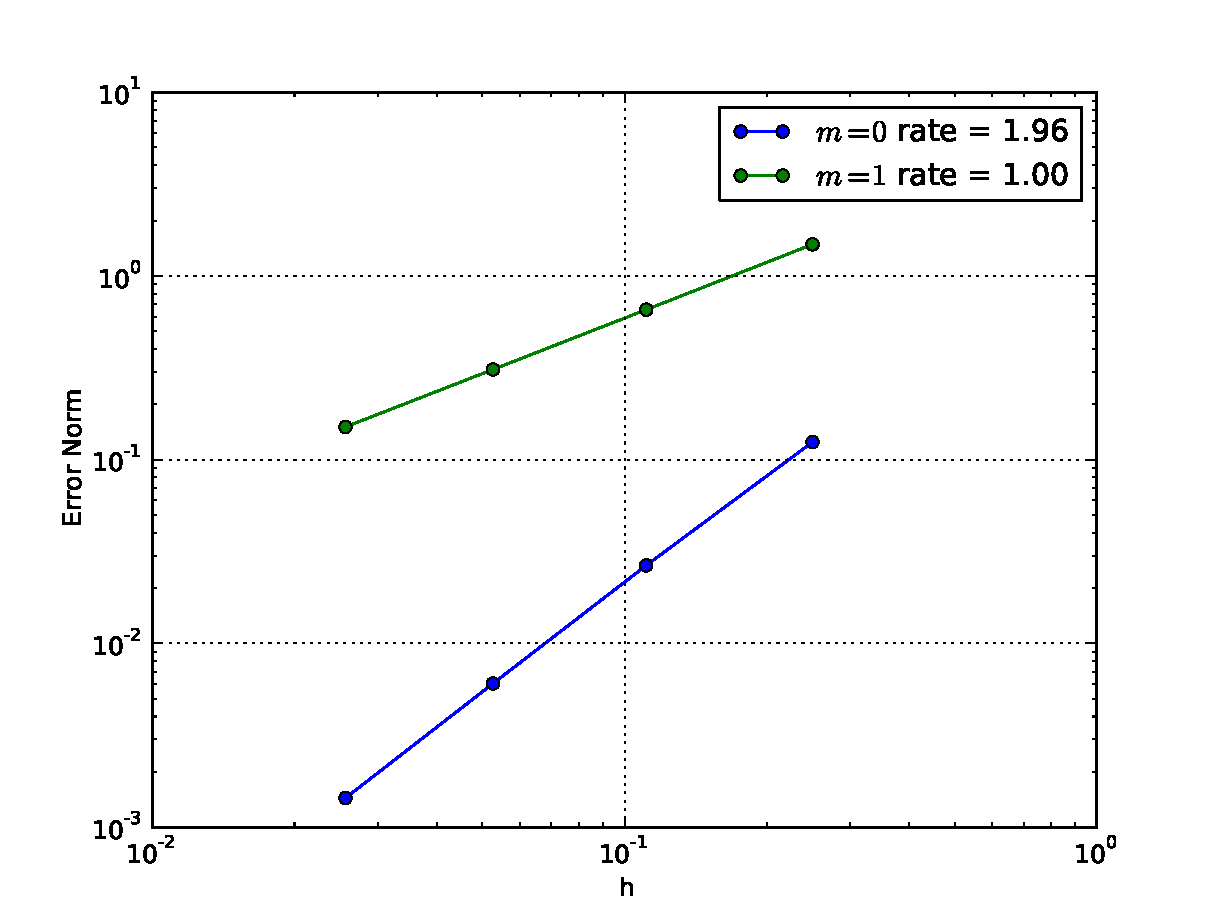
\includegraphics[width=5in]{error.pdf}
\end{center}
\caption{Error norms for $m=0,1$}
\label{fig:error}
\end{figure}

\clearpage
\newpage
\lstinputlisting[language=Python,title={HW10.py}]{HW10.py}

\end{document}
